\documentclass[11pt]{article}
\usepackage[english]{babel}
\usepackage[utf8x]{inputenc}
\usepackage{amsmath}
\usepackage{graphicx}
\usepackage[colorinlistoftodos]{todonotes}
\usepackage{enumitem}
\usepackage{listings}
\usepackage{verbatim}
\usepackage{eurosym}
\usepackage[export]{adjustbox}
\usepackage{amssymb}
\usepackage{bussproofs}
\usepackage{amsmath}
\usepackage{tikz}

%----------------------------------------------------------------------------------------
%	COVER START
%----------------------------------------------------------------------------------------
\begin{document}

    \begin{titlepage}

        \newcommand{\HRule}{\rule{\linewidth}{0.5mm}}
        \newcommand{\department}{Departamento de Matemáticas}
        \newcommand{\course}{Fundamentos de Matemáticas}
        \newcommand{\titleValue}{Quiz Conjuntos y Familias de Conjuntos}
        \newcommand{\subtitleValue}{}
        \newcommand{\authorName}{Alexander Mendoza}

        \center

        %----------------------------------------------------------------------------------------
        %	HEADER
        %----------------------------------------------------------------------------------------

        \vspace{0.5cm}
        \textsc{\Large \department}\\[0.5cm]
        \textsc{\Large \course}\\[0.5cm]
        \vfill

        %----------------------------------------------------------------------------------------
        %	TITLE
        %----------------------------------------------------------------------------------------

        \HRule\\
        \Huge
        \textbf{\titleValue}\\[0.5cm]
        \Large
        \textbf{\subtitleValue}\\
        \HRule\\[0.5cm]

        %----------------------------------------------------------------------------------------
        %	AUTHOR AND DATE
        %----------------------------------------------------------------------------------------

        \vfill
        \Large
        \textit{\authorName}\\
        {\large \today}\\[2cm]

    \end{titlepage}
%----------------------------------------------------------------------------------------
%	COVER END
%----------------------------------------------------------------------------------------
\section*{Quiz}
\begin{enumerate}
    \item Sean $A$ y $B$ subconjuntos de un conjunto $X$, considere la siguiente expresión
        $$
        A \cup B-(A-(A \cap B))
        $$
        \begin{enumerate}
            \item Simplifique la expresión enunciando las propiedades utilizadas.\\
                - La expresión simplificada sería $A \cup B - (A - B)$ esto usando ley de De Morgan.
            \item Realice el diagrama de Venn de la expresión encontrada en el punto anterior.
                \begin{center}
                    \tikzset{every picture/.style={line width=0.75pt}}

                    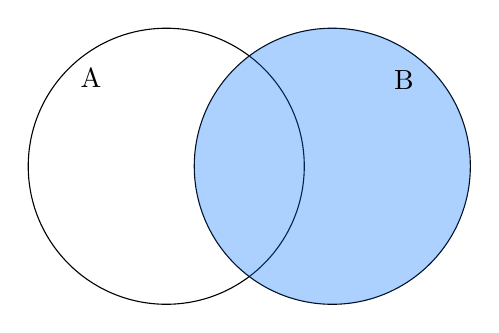
\begin{tikzpicture}[x=0.75pt,y=0.75pt,yscale=-1,xscale=1]
                    \draw   (113,126.5) .. controls (113,89.77) and (142.77,60) .. (179.5,60) .. controls (216.23,60) and (246,89.77) .. (246,126.5) .. controls (246,163.23) and (216.23,193) .. (179.5,193) .. controls (142.77,193) and (113,163.23) .. (113,126.5) -- cycle ;
                    \draw   (193,126.5) .. controls (193,89.77) and (222.77,60) .. (259.5,60) .. controls (296.23,60) and (326,89.77) .. (326,126.5) .. controls (326,163.23) and (296.23,193) .. (259.5,193) .. controls (222.77,193) and (193,163.23) .. (193,126.5) -- cycle ;
                    \draw  [color={rgb, 255:red, 0; green, 0; blue, 0 }  ,draw opacity=0 ][fill={rgb, 255:red, 1; green, 113; blue, 255 }  ,fill opacity=0.32 ] (193,126.5) .. controls (193,89.77) and (222.77,60) .. (259.5,60) .. controls (296.23,60) and (326,89.77) .. (326,126.5) .. controls (326,163.23) and (296.23,193) .. (259.5,193) .. controls (222.77,193) and (193,163.23) .. (193,126.5) -- cycle ;
                    \draw (137,78) node [anchor=north west][inner sep=0.75pt]   [align=left] {A};
                    % Text Node
                    \draw (288,79) node [anchor=north west][inner sep=0.75pt]   [align=left] {B};
                    \end{tikzpicture}
                \end{center}
            \item Con base en el diagrama del item anterior, conjeture a qué es igual la expresión simplificada y demuéstrelo.\\
                - Del diagrama anterior podemos observar que el conjunto resultante es B. \textit{Demostración}. Sabemos que una simplificación de la expresión es $A \cup B - (A - B)$ esto por ley de De Morgan. Luego sea $a \in A$ así $a \in A - B$ por definición de diferencia de conjuntos. Luego sea $b \in B$ así $b \not \in A - B$ por definición de diferencia de conjuntos. Por lo tanto $A \cup B - (A - B) = B$.
        \end{enumerate}
    \item Sean $\mathcal{A}$ y $\mathcal{B}$ dos familias de conjuntos no
    vacías tales que $\mathcal{A} \subseteq \mathcal{B}$. Pruebe que $\bigcap_{B \in \mathcal{B}} B
    \subseteq \bigcap_{A \in \mathcal{A}} A$.\\

        \textit{Demostración}. Sean $\mathcal{A}, \mathcal{B}$ familias de conjuntos tal que $\mathcal{A} \subseteq \mathcal{B}$ y sea $c \in B$ para todo $B \in \mathcal{B}$, luego $c \in A$ para todo $A \in \mathcal{A}$ esto por definición de subconjunto. Luego $c \in \bigcap_{B \in \mathcal{B}}$ por definición de intersección de familia de conjuntos. Por lo tanto $c \in \bigcap_{A \in \mathcal{A}} A$, así $\bigcap_{B \in \mathcal{B}} B \subseteq \bigcap_{A \in \mathcal{A}} A$ por definición de subconjunto.
\end{enumerate}
\end{document}